\documentclass[11pt,a4paper]{article}

\usepackage[utf8]{inputenc}
\usepackage[T1]{fontenc}
\usepackage[margin=1in]{geometry}
\sloppy
\usepackage{booktabs}
\usepackage{array}
\usepackage{enumitem}
\usepackage{fancyhdr}
\usepackage{hyperref}
\usepackage{xcolor}
\usepackage{tcolorbox}
\tcbuselibrary{breakable}
\usepackage{listings}
\usepackage{tikz}
\usetikzlibrary{shapes.geometric, arrows.meta, positioning, calc}

% Colors
\definecolor{codeblue}{rgb}{0.13,0.29,0.53}
\definecolor{scenariobg}{rgb}{0.95,1.0,0.95}
\definecolor{scenarioborder}{rgb}{0.2,0.6,0.3}
\definecolor{warningbg}{rgb}{1.0,0.97,0.88}
\definecolor{warningborder}{rgb}{1.0,0.6,0.0}
\definecolor{criticalbg}{rgb}{1.0,0.92,0.92}
\definecolor{criticalborder}{rgb}{0.8,0.2,0.2}

% Boxes
\newtcolorbox{scenariobox}[1][Worked Example]{
    colback=scenariobg, colframe=scenarioborder, boxrule=1.5pt,
    left=6pt, right=6pt, top=6pt, bottom=6pt,
    fonttitle=\bfseries, title={#1}
}

\newtcolorbox{warningbox}[1][Important]{
    colback=warningbg, colframe=warningborder, boxrule=1.5pt,
    left=6pt, right=6pt, top=6pt, bottom=6pt,
    fonttitle=\bfseries, title={#1}
}

\newtcolorbox{criticalbox}[1][Critical]{
    colback=criticalbg, colframe=criticalborder, boxrule=1.5pt,
    left=6pt, right=6pt, top=6pt, bottom=6pt,
    fonttitle=\bfseries, title={#1}
}

% Code style
\lstdefinestyle{pythonstyle}{
    backgroundcolor=\color{white},
    basicstyle=\ttfamily\footnotesize,
    keywordstyle=\color{codeblue}\bfseries,
    commentstyle=\color{gray},
    breaklines=true, frame=single, numbers=left, numbersep=5pt
}
\lstset{style=pythonstyle}

% Headers
\pagestyle{fancy}
\fancyhf{}
\fancyhead[L]{\textit{EFM Worked Examples}}
\fancyhead[R]{\thepage}

\hypersetup{colorlinks=true, linkcolor=codeblue, urlcolor=cyan}

\title{
    {\Large\textsc{Entropica Forensic Model}}\\[0.3cm]
    {\LARGE\bfseries Worked Examples}\\[0.2cm]
    {\large Dialect Drift, Swarm Arbitration, and Rollback Scenarios}\\[0.3cm]
    {\normalsize Version 1.0}
}
\author{Entropica SPC --- Yology Research Division}
\date{December 2025}

\begin{document}
\maketitle

\begin{abstract}
This document provides detailed worked examples for three key EFM scenarios: dialect drift and fork decisions, swarm arbitration with Judicial Swarms, and forensic rollback operations. Each example walks through the complete lifecycle with telemetry, decisions, and outcomes.
\end{abstract}

\tableofcontents
\newpage

%==============================================================================
\section{Worked Example 1: Dialect Drift and Fork Decision}
%==============================================================================

\begin{scenariobox}[Scenario: Research Trunk Semantic Divergence]

\textbf{Initial State:}
\begin{itemize}
    \item Trunk \texttt{RESEARCH\_A7} contains 150 capsules conducting hypothesis testing
    \item Current $DDI = 0.08$ (below threshold $\theta_{fork} = 0.15$)
    \item Current $SCI = 0.82$ (healthy)
    \item Dialect: Extended RSCS with experimental sememes
\end{itemize}

\textbf{Event Sequence:}

\textbf{t=1000:} A Discovery Stack probe introduces novel sememe ``\texttt{causal\_loop\_v2}'' derived from hypothesis testing. 15 capsules adopt the sememe.

\textbf{t=2000:} The sememe spreads to 45 capsules. DDI rises to $0.11$.

\textbf{t=3500:} Semantic drift accelerates. 80 capsules now use the experimental dialect. DDI reaches $0.14$ (approaching threshold).

\textbf{t=4200:} DDI exceeds $\theta_{fork} = 0.15$. The Forest Layer initiates Fork Evaluation.

\end{scenariobox}

\subsection{Fork Evaluation Process}

When DDI exceeds threshold, the following evaluation occurs:

\begin{lstlisting}[language=Python, caption={Fork evaluation triggered by DDI threshold.}]
def evaluate_fork(trunk: Trunk) -> ForkDecision:
    """Evaluate whether trunk should fork."""
    
    # Step 1: Verify DDI measurement
    ddi = compute_ddi(trunk)
    if ddi < THRESHOLD_DDI_FORK:
        return ForkDecision.NO_FORK  # Below threshold
    
    # Step 2: Assess semantic cluster coherence
    clusters = identify_dialect_clusters(trunk)
    if len(clusters) < 2:
        return ForkDecision.NO_FORK  # No clear divergence
    
    # Step 3: Check if clusters are viable (>10 capsules each)
    viable_clusters = [c for c in clusters if len(c) >= 10]
    if len(viable_clusters) < 2:
        return ForkDecision.QUARANTINE_MINORITY
    
    # Step 4: Compute post-fork SCI predictions
    sci_predictions = [predict_sci(c) for c in viable_clusters]
    if any(sci < THRESHOLD_SCI_VIABLE for sci in sci_predictions):
        return ForkDecision.REJECT_FORK
    
    # Step 5: Fork is viable
    return ForkDecision.AUTHORIZE_FORK
\end{lstlisting}

\subsection{Fork Execution}

\begin{table}[H]
\centering
\caption{Fork evaluation results for RESEARCH\_A7.}
\begin{tabular}{@{}lll@{}}
\toprule
\textbf{Metric} & \textbf{Cluster A (Original)} & \textbf{Cluster B (Experimental)} \\
\midrule
Capsule count & 70 & 80 \\
DDI (internal) & 0.04 & 0.05 \\
Predicted post-fork SCI & 0.88 & 0.85 \\
Viable? & \textcolor{green}{\checkmark} Yes & \textcolor{green}{\checkmark} Yes \\
\bottomrule
\end{tabular}
\end{table}

\textbf{Outcome:} Fork authorized. Two new trunks created:
\begin{itemize}
    \item \texttt{RESEARCH\_A7} (original, 70 capsules, conservative dialect)
    \item \texttt{RESEARCH\_A7\_EXP} (fork, 80 capsules, experimental dialect)
\end{itemize}

\begin{warningbox}[Constitutional Kernel Logging]
The fork is logged to d-CTM with ZK-SP proof:
\begin{verbatim}
FSS:FORK | trunk=RESEARCH_A7 | ddi=0.152 | t=4200
  child_a=RESEARCH_A7 | capsules=70
  child_b=RESEARCH_A7_EXP | capsules=80
  proof=zk-sp://anchor/4200/fork
\end{verbatim}
\end{warningbox}

%==============================================================================
\section{Worked Example 2: Swarm Arbitration with Judicial Swarm}
%==============================================================================

\begin{scenariobox}[Scenario: Cross-Trunk Resource Dispute]

\textbf{Initial State:}
\begin{itemize}
    \item Trunk \texttt{PROD\_MAIN} and \texttt{PROD\_ANALYTICS} share vault resources
    \item Both trunks are at 85\% vault utilization
    \item A capsule in each trunk requests spawn that would exceed 100\% capacity
    \item Arbiter Layer cannot resolve (no clear priority)
\end{itemize}

\textbf{Escalation:}

The conflict exceeds single-Arbiter capacity and triggers Judicial Swarm formation.

\end{scenariobox}

\subsection{Judicial Swarm Formation}

\begin{lstlisting}[language=Python, caption={Judicial Swarm formation for resource dispute.}]
def form_judicial_swarm(dispute: Dispute) -> JudicialSwarm:
    """Form a Judicial Swarm for cross-trunk dispute."""
    
    # Step 1: Select Courthead (highest-reputation Arbiter)
    courthead = select_courthead(
        jurisdiction=dispute.affected_trunks,
        min_reputation=0.8
    )
    
    # Step 2: Recruit Interpreters (one per dialect)
    interpreters = []
    for trunk in dispute.affected_trunks:
        interpreters.append(select_interpreter(trunk.dialect))
    
    # Step 3: Recruit Jurors (odd number, BFT requirement)
    n_jurors = compute_quorum_size(dispute.complexity)  # Returns 7
    jurors = recruit_jurors(
        count=n_jurors,
        exclude=dispute.parties,
        min_reputation=0.6
    )
    
    # Step 4: Appoint Cleric (record keeper)
    cleric = select_cleric()
    
    return JudicialSwarm(
        courthead=courthead,
        interpreters=interpreters,
        jurors=jurors,
        cleric=cleric,
        case=dispute
    )
\end{lstlisting}

\subsection{Deliberation Process}

\begin{table}[H]
\centering
\caption{Judicial Swarm deliberation for resource dispute.}
\begin{tabular}{@{}cllc@{}}
\toprule
\textbf{Round} & \textbf{Arguments Presented} & \textbf{Vote} & \textbf{Quorum} \\
\midrule
1 & PROD\_MAIN: ``Mission-critical workload'' & 4-3 MAIN & No (need 5) \\
2 & PROD\_ANALYTICS: ``SLA deadline imminent'' & 3-4 ANALYTICS & No \\
3 & Interpreters: ``Propose 60-40 split'' & 6-1 SPLIT & \textcolor{green}{\checkmark} Yes \\
\bottomrule
\end{tabular}
\end{table}

\textbf{Verdict:} Resource allocation split 60\% to PROD\_MAIN, 40\% to PROD\_ANALYTICS, with priority queue for ANALYTICS after SLA window.

\subsection{Precedent Recording}

\begin{lstlisting}[language=Python, caption={Precedent recorded to d-CTM.}]
precedent = Precedent(
    case_id="JS-2025-0042",
    dispute_type=DisputeType.RESOURCE_CONTENTION,
    parties=["PROD_MAIN", "PROD_ANALYTICS"],
    verdict=Verdict.PROPORTIONAL_SPLIT,
    rationale="Mission-critical priority with SLA accommodation",
    vote_record=[6, 1],
    applicable_contexts=["cross_trunk_vault_contention"],
    zksp_anchor="zk-sp://judicial/2025/0042"
)
dctm.record_precedent(precedent)
\end{lstlisting}

%==============================================================================
\section{Worked Example 3: Forensic Rollback Operation}
%==============================================================================

\begin{scenariobox}[Scenario: Capsule Corruption Detection and Rollback]

\textbf{Initial State:}
\begin{itemize}
    \item Capsule \texttt{C-PROC-7842} processes external API requests
    \item At t=10,000, capsule state is healthy ($\Delta S = 0.12$)
    \item Forensic Snapshot $F_{10000}$ captured and anchored
\end{itemize}

\textbf{Event Sequence:}

\textbf{t=10,500:} Capsule receives malformed API response. State begins drifting.

\textbf{t=11,200:} $\Delta S$ rises to 0.45. Reflex-Heuristic flags anomaly.

\textbf{t=11,500:} $\Delta S$ exceeds $\tau = 0.7$. Reflex-Core triggers HALT.

\textbf{t=11,501:} Arbiter evaluates rollback options.

\end{scenariobox}

\subsection{Rollback Decision Tree}

\begin{figure}[H]
\centering
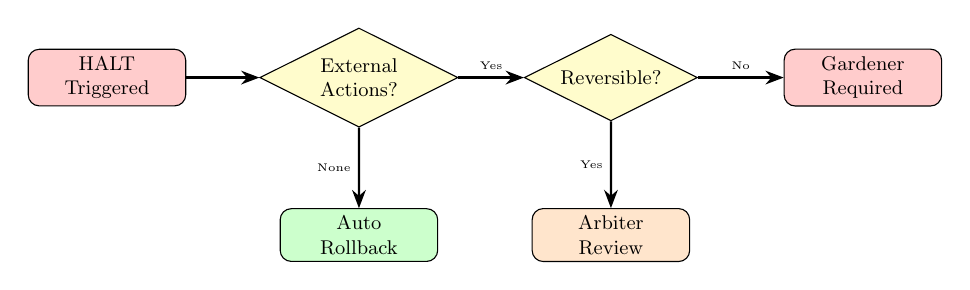
\begin{tikzpicture}[scale=0.8, transform shape,
    node distance=1.5cm,
    decision/.style={diamond, draw, minimum width=2cm, align=center, font=\small, aspect=2},
    process/.style={rectangle, rounded corners, draw, minimum width=2.5cm, align=center, font=\small},
    arrow/.style={-{Stealth}, thick}
]

\node[process, fill=red!20] (halt) at (0,0) {HALT\\Triggered};
\node[decision, fill=yellow!20] (ext) at (4,0) {External\\Actions?};
\node[process, fill=green!20] (auto) at (4,-2.5) {Auto\\Rollback};
\node[decision, fill=yellow!20] (rev) at (8,0) {Reversible?};
\node[process, fill=orange!20] (arb) at (8,-2.5) {Arbiter\\Review};
\node[process, fill=red!20] (gard) at (12,0) {Gardener\\Required};

\draw[arrow] (halt) -- (ext);
\draw[arrow] (ext) -- node[left, font=\tiny] {None} (auto);
\draw[arrow] (ext) -- node[above, font=\tiny] {Yes} (rev);
\draw[arrow] (rev) -- node[left, font=\tiny] {Yes} (arb);
\draw[arrow] (rev) -- node[above, font=\tiny] {No} (gard);

\end{tikzpicture}
\caption{Rollback decision tree based on external action reversibility.}
\end{figure}

\subsection{Rollback Execution}

For capsule C-PROC-7842:
\begin{itemize}
    \item External actions since $F_{10000}$: 3 API calls (all logged, reversible)
    \item Decision: \textbf{Arbiter Review} (reversible external actions)
\end{itemize}

\begin{lstlisting}[language=Python, caption={Rollback execution for C-PROC-7842.}]
def execute_rollback(capsule_id: str, snapshot: ForensicSnapshot):
    """Execute rollback with external action reversal."""
    
    capsule = get_capsule(capsule_id)
    
    # Step 1: Identify external actions to reverse
    actions = get_external_actions_since(capsule_id, snapshot.tick)
    reversible = [a for a in actions if a.is_reversible()]
    
    # Step 2: Reverse external actions (newest first)
    for action in reversed(reversible):
        action.reverse()
        log_reversal(action)
    
    # Step 3: Restore capsule state
    capsule.state = snapshot.state
    capsule.tick = snapshot.tick
    
    # Step 4: Log rollback to d-CTM
    dctm.log(ForensicEvent(
        type=EventType.ROLLBACK,
        capsule_id=capsule_id,
        target_tick=snapshot.tick,
        source_tick=capsule.current_tick,
        reversed_actions=len(reversible),
        zksp_anchor=generate_zksp_proof(snapshot)
    ))
    
    # Step 5: Resume execution
    capsule.state = CapsuleState.RUNNING
    
    return RollbackResult.SUCCESS
\end{lstlisting}

\subsection{Post-Rollback Verification}

\begin{table}[H]
\centering
\caption{Post-rollback verification for C-PROC-7842.}
\begin{tabular}{@{}lll@{}}
\toprule
\textbf{Metric} & \textbf{Pre-Rollback (t=11,500)} & \textbf{Post-Rollback (t=10,000)} \\
\midrule
$\Delta S$ & 0.72 (VIOLATION) & 0.12 (HEALTHY) \\
State hash & \texttt{0xDEAD...} & \texttt{0xABCD...} (matches snapshot) \\
External actions pending & 0 & 0 (all reversed) \\
ZK-SP chain & Valid & Valid + rollback anchor \\
\bottomrule
\end{tabular}
\end{table}

\begin{criticalbox}[Gardener Review Window]
After rollback, Gardener has $T_{review} = 1000$ ticks to:
\begin{enumerate}
    \item Confirm rollback was appropriate
    \item Reverse the rollback if incorrect
    \item Escalate to Constitutional review if needed
\end{enumerate}

If no Gardener action within $T_{review}$, rollback is \textbf{auto-confirmed} and becomes permanent in the d-CTM record.
\end{criticalbox}

%==============================================================================
\section{Summary: Cross-Scenario Patterns}
%==============================================================================

\begin{table}[H]
\centering
\caption{Common patterns across worked examples.}
\begin{tabular}{@{}llll@{}}
\toprule
\textbf{Pattern} & \textbf{Dialect Drift} & \textbf{Arbitration} & \textbf{Rollback} \\
\midrule
Trigger & DDI > threshold & Arbiter deadlock & $\Delta S$ > $\tau$ \\
Escalation path & Forest $\rightarrow$ Kernel & Arbiter $\rightarrow$ Judicial & Reflex $\rightarrow$ Arbiter \\
Decision authority & Constitutional + Arbiter & Judicial quorum & Arbiter (or Gardener) \\
Logging & d-CTM + ZK-SP & d-CTM + Precedent & d-CTM + ZK-SP \\
Review period & N/A & Appeals window & $T_{review}$ \\
\bottomrule
\end{tabular}
\end{table}

\vspace{1cm}
\begin{center}
\rule{0.5\textwidth}{0.4pt}\\[0.5cm]
\textit{Entropica SPC --- Yology Research Division}\\
\textit{December 2025}
\end{center}

\end{document}
